% Created by tikzDevice version 0.12.3.1 on 2021-07-13 22:52:15
% !TEX encoding = UTF-8 Unicode
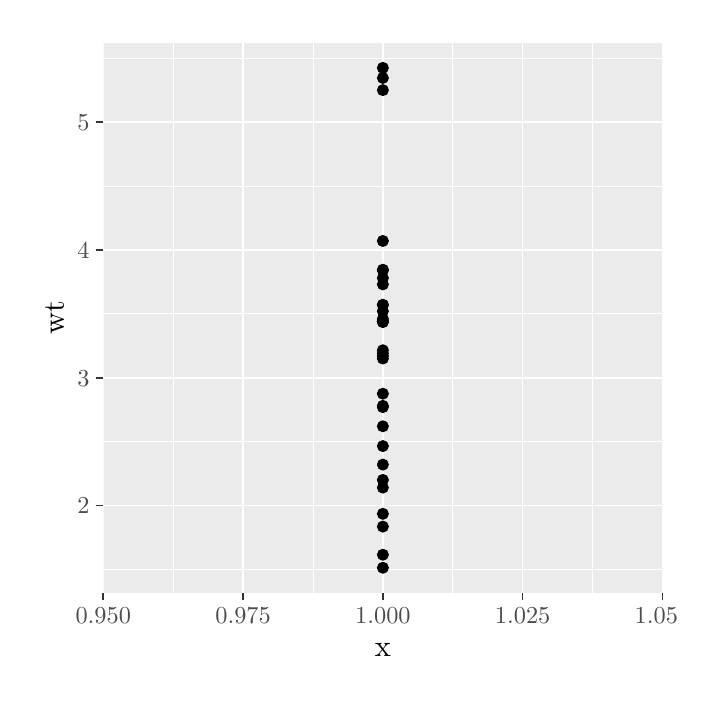
\begin{tikzpicture}[x=1pt,y=1pt]
\definecolor{fillColor}{RGB}{255,255,255}
\path[use as bounding box,fill=fillColor,fill opacity=0.00] (0,0) rectangle (234.88,234.88);
\begin{scope}
\path[clip] (  0.00,  0.00) rectangle (234.88,234.88);
\definecolor{drawColor}{RGB}{255,255,255}
\definecolor{fillColor}{RGB}{255,255,255}

\path[draw=drawColor,line width= 0.6pt,line join=round,line cap=round,fill=fillColor] (  0.00,  0.00) rectangle (234.88,234.88);
\end{scope}
\begin{scope}
\path[clip] ( 27.31, 30.69) rectangle (229.38,229.38);
\definecolor{fillColor}{gray}{0.92}

\path[fill=fillColor] ( 27.31, 30.69) rectangle (229.38,229.38);
\definecolor{drawColor}{RGB}{255,255,255}

\path[draw=drawColor,line width= 0.3pt,line join=round] ( 27.31, 39.12) --
	(229.38, 39.12);

\path[draw=drawColor,line width= 0.3pt,line join=round] ( 27.31, 85.30) --
	(229.38, 85.30);

\path[draw=drawColor,line width= 0.3pt,line join=round] ( 27.31,131.49) --
	(229.38,131.49);

\path[draw=drawColor,line width= 0.3pt,line join=round] ( 27.31,177.67) --
	(229.38,177.67);

\path[draw=drawColor,line width= 0.3pt,line join=round] ( 27.31,223.86) --
	(229.38,223.86);

\path[draw=drawColor,line width= 0.3pt,line join=round] ( 52.57, 30.69) --
	( 52.57,229.38);

\path[draw=drawColor,line width= 0.3pt,line join=round] (103.09, 30.69) --
	(103.09,229.38);

\path[draw=drawColor,line width= 0.3pt,line join=round] (153.60, 30.69) --
	(153.60,229.38);

\path[draw=drawColor,line width= 0.3pt,line join=round] (204.12, 30.69) --
	(204.12,229.38);

\path[draw=drawColor,line width= 0.6pt,line join=round] ( 27.31, 62.21) --
	(229.38, 62.21);

\path[draw=drawColor,line width= 0.6pt,line join=round] ( 27.31,108.39) --
	(229.38,108.39);

\path[draw=drawColor,line width= 0.6pt,line join=round] ( 27.31,154.58) --
	(229.38,154.58);

\path[draw=drawColor,line width= 0.6pt,line join=round] ( 27.31,200.76) --
	(229.38,200.76);

\path[draw=drawColor,line width= 0.6pt,line join=round] ( 27.31, 30.69) --
	( 27.31,229.38);

\path[draw=drawColor,line width= 0.6pt,line join=round] ( 77.83, 30.69) --
	( 77.83,229.38);

\path[draw=drawColor,line width= 0.6pt,line join=round] (128.35, 30.69) --
	(128.35,229.38);

\path[draw=drawColor,line width= 0.6pt,line join=round] (178.86, 30.69) --
	(178.86,229.38);

\path[draw=drawColor,line width= 0.6pt,line join=round] (229.38, 30.69) --
	(229.38,229.38);
\definecolor{drawColor}{RGB}{0,0,0}
\definecolor{fillColor}{RGB}{0,0,0}

\path[draw=drawColor,line width= 0.4pt,line join=round,line cap=round,fill=fillColor] (128.35, 90.84) circle (  1.96);

\path[draw=drawColor,line width= 0.4pt,line join=round,line cap=round,fill=fillColor] (128.35,102.62) circle (  1.96);

\path[draw=drawColor,line width= 0.4pt,line join=round,line cap=round,fill=fillColor] (128.35, 76.99) circle (  1.96);

\path[draw=drawColor,line width= 0.4pt,line join=round,line cap=round,fill=fillColor] (128.35,118.32) circle (  1.96);

\path[draw=drawColor,line width= 0.4pt,line join=round,line cap=round,fill=fillColor] (128.35,128.72) circle (  1.96);

\path[draw=drawColor,line width= 0.4pt,line join=round,line cap=round,fill=fillColor] (128.35,129.64) circle (  1.96);

\path[draw=drawColor,line width= 0.4pt,line join=round,line cap=round,fill=fillColor] (128.35,134.72) circle (  1.96);

\path[draw=drawColor,line width= 0.4pt,line join=round,line cap=round,fill=fillColor] (128.35,117.17) circle (  1.96);

\path[draw=drawColor,line width= 0.4pt,line join=round,line cap=round,fill=fillColor] (128.35,115.32) circle (  1.96);

\path[draw=drawColor,line width= 0.4pt,line join=round,line cap=round,fill=fillColor] (128.35,128.72) circle (  1.96);

\path[draw=drawColor,line width= 0.4pt,line join=round,line cap=round,fill=fillColor] (128.35,128.72) circle (  1.96);

\path[draw=drawColor,line width= 0.4pt,line join=round,line cap=round,fill=fillColor] (128.35,157.81) circle (  1.96);

\path[draw=drawColor,line width= 0.4pt,line join=round,line cap=round,fill=fillColor] (128.35,142.11) circle (  1.96);

\path[draw=drawColor,line width= 0.4pt,line join=round,line cap=round,fill=fillColor] (128.35,144.42) circle (  1.96);

\path[draw=drawColor,line width= 0.4pt,line join=round,line cap=round,fill=fillColor] (128.35,212.31) circle (  1.96);

\path[draw=drawColor,line width= 0.4pt,line join=round,line cap=round,fill=fillColor] (128.35,220.35) circle (  1.96);

\path[draw=drawColor,line width= 0.4pt,line join=round,line cap=round,fill=fillColor] (128.35,216.70) circle (  1.96);

\path[draw=drawColor,line width= 0.4pt,line join=round,line cap=round,fill=fillColor] (128.35, 71.45) circle (  1.96);

\path[draw=drawColor,line width= 0.4pt,line join=round,line cap=round,fill=fillColor] (128.35, 44.43) circle (  1.96);

\path[draw=drawColor,line width= 0.4pt,line join=round,line cap=round,fill=fillColor] (128.35, 54.59) circle (  1.96);

\path[draw=drawColor,line width= 0.4pt,line join=round,line cap=round,fill=fillColor] (128.35, 83.69) circle (  1.96);

\path[draw=drawColor,line width= 0.4pt,line join=round,line cap=round,fill=fillColor] (128.35,132.41) circle (  1.96);

\path[draw=drawColor,line width= 0.4pt,line join=round,line cap=round,fill=fillColor] (128.35,128.48) circle (  1.96);

\path[draw=drawColor,line width= 0.4pt,line join=round,line cap=round,fill=fillColor] (128.35,147.19) circle (  1.96);

\path[draw=drawColor,line width= 0.4pt,line join=round,line cap=round,fill=fillColor] (128.35,147.42) circle (  1.96);

\path[draw=drawColor,line width= 0.4pt,line join=round,line cap=round,fill=fillColor] (128.35, 59.21) circle (  1.96);

\path[draw=drawColor,line width= 0.4pt,line join=round,line cap=round,fill=fillColor] (128.35, 68.68) circle (  1.96);

\path[draw=drawColor,line width= 0.4pt,line join=round,line cap=round,fill=fillColor] (128.35, 39.72) circle (  1.96);

\path[draw=drawColor,line width= 0.4pt,line join=round,line cap=round,fill=fillColor] (128.35,116.25) circle (  1.96);

\path[draw=drawColor,line width= 0.4pt,line join=round,line cap=round,fill=fillColor] (128.35, 97.77) circle (  1.96);

\path[draw=drawColor,line width= 0.4pt,line join=round,line cap=round,fill=fillColor] (128.35,134.72) circle (  1.96);

\path[draw=drawColor,line width= 0.4pt,line join=round,line cap=round,fill=fillColor] (128.35, 98.23) circle (  1.96);
\end{scope}
\begin{scope}
\path[clip] (  0.00,  0.00) rectangle (234.88,234.88);
\definecolor{drawColor}{gray}{0.30}

\node[text=drawColor,anchor=base east,inner sep=0pt, outer sep=0pt, scale=  0.88] at ( 22.36, 59.18) {2};

\node[text=drawColor,anchor=base east,inner sep=0pt, outer sep=0pt, scale=  0.88] at ( 22.36,105.36) {3};

\node[text=drawColor,anchor=base east,inner sep=0pt, outer sep=0pt, scale=  0.88] at ( 22.36,151.55) {4};

\node[text=drawColor,anchor=base east,inner sep=0pt, outer sep=0pt, scale=  0.88] at ( 22.36,197.73) {5};
\end{scope}
\begin{scope}
\path[clip] (  0.00,  0.00) rectangle (234.88,234.88);
\definecolor{drawColor}{gray}{0.20}

\path[draw=drawColor,line width= 0.6pt,line join=round] ( 24.56, 62.21) --
	( 27.31, 62.21);

\path[draw=drawColor,line width= 0.6pt,line join=round] ( 24.56,108.39) --
	( 27.31,108.39);

\path[draw=drawColor,line width= 0.6pt,line join=round] ( 24.56,154.58) --
	( 27.31,154.58);

\path[draw=drawColor,line width= 0.6pt,line join=round] ( 24.56,200.76) --
	( 27.31,200.76);
\end{scope}
\begin{scope}
\path[clip] (  0.00,  0.00) rectangle (234.88,234.88);
\definecolor{drawColor}{gray}{0.20}

\path[draw=drawColor,line width= 0.6pt,line join=round] ( 27.31, 27.94) --
	( 27.31, 30.69);

\path[draw=drawColor,line width= 0.6pt,line join=round] ( 77.83, 27.94) --
	( 77.83, 30.69);

\path[draw=drawColor,line width= 0.6pt,line join=round] (128.35, 27.94) --
	(128.35, 30.69);

\path[draw=drawColor,line width= 0.6pt,line join=round] (178.86, 27.94) --
	(178.86, 30.69);

\path[draw=drawColor,line width= 0.6pt,line join=round] (229.38, 27.94) --
	(229.38, 30.69);
\end{scope}
\begin{scope}
\path[clip] (  0.00,  0.00) rectangle (234.88,234.88);
\definecolor{drawColor}{gray}{0.30}

\node[text=drawColor,anchor=base,inner sep=0pt, outer sep=0pt, scale=  0.88] at ( 27.31, 19.68) {0.950};

\node[text=drawColor,anchor=base,inner sep=0pt, outer sep=0pt, scale=  0.88] at ( 77.83, 19.68) {0.975};

\node[text=drawColor,anchor=base,inner sep=0pt, outer sep=0pt, scale=  0.88] at (128.35, 19.68) {1.000};

\node[text=drawColor,anchor=base,inner sep=0pt, outer sep=0pt, scale=  0.88] at (178.86, 19.68) {1.025};

\node[text=drawColor,anchor=base,inner sep=0pt, outer sep=0pt, scale=  0.88] at (229.38, 19.68) {1.050};
\end{scope}
\begin{scope}
\path[clip] (  0.00,  0.00) rectangle (234.88,234.88);
\definecolor{drawColor}{RGB}{0,0,0}

\node[text=drawColor,anchor=base,inner sep=0pt, outer sep=0pt, scale=  1.10] at (128.35,  7.64) {x};
\end{scope}
\begin{scope}
\path[clip] (  0.00,  0.00) rectangle (234.88,234.88);
\definecolor{drawColor}{RGB}{0,0,0}

\node[text=drawColor,rotate= 90.00,anchor=base,inner sep=0pt, outer sep=0pt, scale=  1.10] at ( 13.08,130.03) {wt};
\end{scope}
\end{tikzpicture}
